\section{Measurements}
\label{sec:measurements} 
\subsection{Measurement 2.1: Uranium}
\label{subsec:uranium}
We chose a range from 1000V to 4000V with a stepsize of 100V, whereas each step was measured 100s. 
For the estimation of the error we used the error on the number of counts $N$ by
\begin{equation}
n = \frac{N}{T} \qquad \Rightarrow \qquad s_n =\sqrt{\left ( \frac{\partial n}{\partial N} s_N \right )^2 + \left (\frac{\partial n}{\partial t}s_t \right)^2 }
\approx \frac{\sqrt{N}}{t} = \sqrt{\frac{n}{t}}
\label{eq:error}
\end{equation}
with $S_N=\sqrt{N}$, implying a poissonian process and neglecting the error on $s_N$.
First we measured the radiative uranium preperation while varying the 
applied voltage, see \textbf{figure~\ref{fig:2_1_uranium}} for the visualization 
of the data. We can differentiate very well the two plateaus;
the $\alpha$ plateau from 1500V to 2500V and the  $\beta$ plateau from about 3000V to 4000V.
\begin{figure}[H]
    \centering
    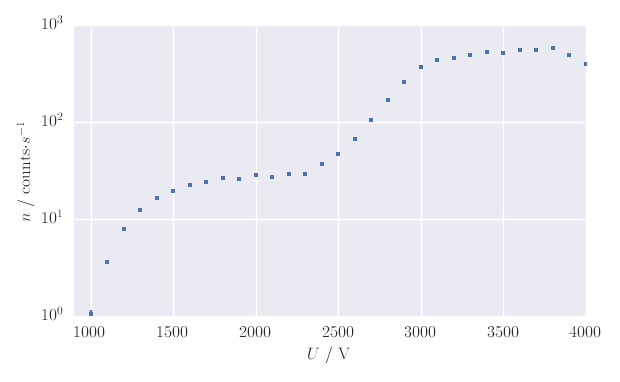
\includegraphics[width=\linewidth]{analysis/figures/2_1_uranium}
    \caption{Measurement 2.1 of an uranium $\mathrm{~^{238}_{92}U}$ sample. We chose a range from 1000V to 4000V
    with a stepsize of 100V, whereas each step was measured 100s. As estimation for the
    error we used $s_n=\sqrt{n / t}$, which is explained within the text in formula \eqref{eq:error}. In this figure 
    we already subtracted the background, see \textbf{figure~\ref{fig:2_2_background2}}. Since 
    the error is orders of magnitude smaller, we can neglect the additional error coming from subtracting the background. }
    \label{fig:2_1_uranium}
\end{figure}
\subsection{Measurement 2.2: Background}
\label{subsec:background}
\begin{figure}[H]
    \centering
    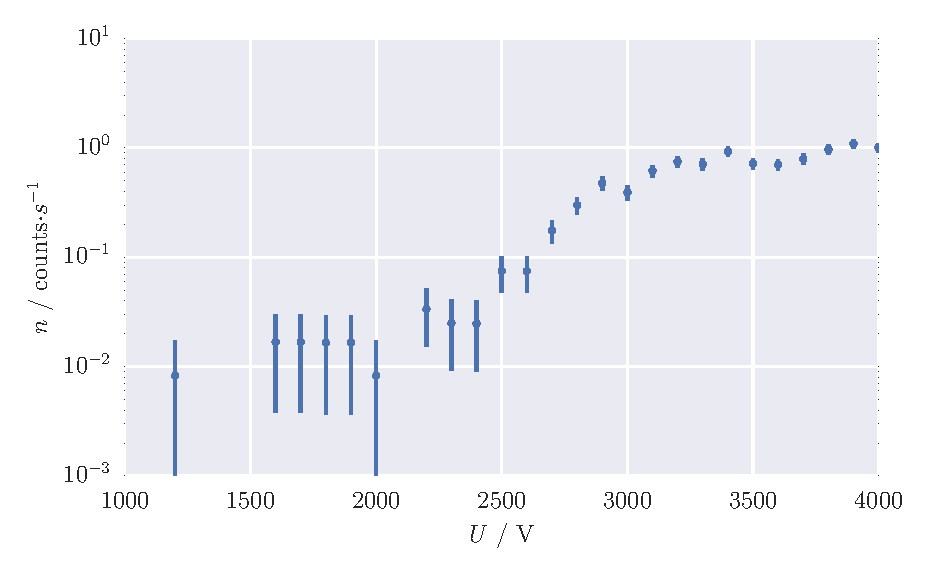
\includegraphics[width=\linewidth]{analysis/figures/2_2_background2}
    \caption{Measurement 2.2 of an the background. We chose the same configuration as in measurement 2.1 with uranium, see
    \textbf{figure~\ref{fig:2_1_uranium}}.}
    \label{fig:2_2_background2}
\end{figure}

In order to estimate the order of magnitude of the background we measured without any radiactive preperation, for 
the visualization see \textbf{figure~\ref{fig:2_2_background2}}. This was the measurement with varying voltage.
We also conducted a measurement at the working points $U_{sam} = 2000$V for samarium (subsection~\ref{subsec:samarium}) and
$U_{pot} = 3500$V for potassium (subsection~\ref{subsec:potassium}). The result can be viewed in tables~\ref{tab:background_night1}.
\begin{SCtable}

\centering
\begin{tabular}{ll}
 \rowcolor{tabcolor}$U$ & $2000$ V (Working point samarium)\\
 $U_{step}$ & 1500 V \\
 \rowcolor{tabcolor}$\Delta t$ & 25000s = 6 hours \\
 $\bar{n}$ & $\left [ 0.0074 \pm 0.0005 \right ] \text{counts} \cdot s^{-1}$ \\
  \\
 \rowcolor{tabcolor}$U$ & $3500$ V (Working point potassium)\\
 $U_{step}$ & 1500 V \\
 \rowcolor{tabcolor}$\Delta t$ & 25000s = 6 hours \\
 $\bar{n}$ & $\left [ 0.451 \pm 0.004 \right ] \text{counts} \cdot s^{-1}$ \\
 \end{tabular}

\caption{Measurements from the background. The error was calculated for each with
$s_n = \sqrt{\frac{n}{t}}$ which was calculated in equation~\ref{eq:error}.
}
\label{tab:background_night1}

\end{SCtable}
\subsection{Measurement 2.3: Samarium}
\label{subsec:samarium}
In order to visualize the $\alpha$ plateau for finding the working point we chose a range of 1000V to 3500V with a stepsize of 100V and 
a time per step of 200 s. In this case the samarium activity is in same order of magnitude of the 
background, therefore we have to compare the errors of samarium $n_{sam}$ and the background $n_{back}$
\begin{equation}
    n_{total} = n_{sam.} - n_{back.} \Rightarrow  s_{n,total} 
    =\sqrt{\left( \frac{\partial n_{sam.}}{\partial N} s_N \right )^2+\left (\frac{\partial n_{back.}}{\partial N} s_N \right )^2 } 
    = \sqrt{\frac{n_{sam.}}{t_{sam.}}+\frac{u_{back.}}{t_{back.}} }
    \label{eq:error_sam}
\end{equation}
This error will become quite big in the evaluation, see figure~\ref{fig:2_3_samarium} for the visualization when we subtracted the
background and without subtracting. Following from this figure, we decided to choose the working point to be
\begin{equation}
U_{ref} = 2000 \mathrm{V}.
\end{equation}
\begin{figure}[H]
    \centering
    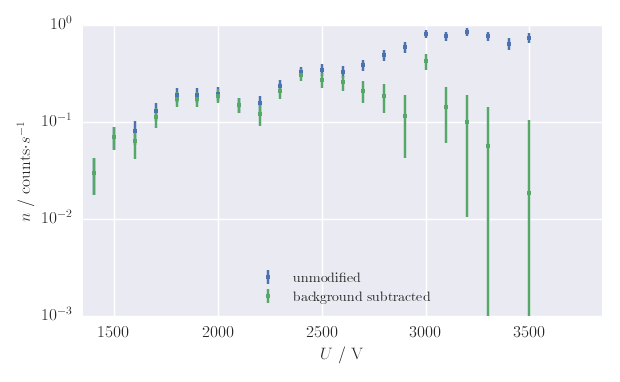
\includegraphics[width=\linewidth]{analysis/figures/measurement_2_2_1}
    \caption{Measurement 2.3 of samarium, where the blue bars denote to the unmodified samarium signal and the blue bars to the
    samarium signal from which the background has been subtracted.
    The error was chosen with $s_n = \sqrt{\frac{n_{sam.}}{t_{sam.}}+\frac{u_{back.}}{t_{back.}} }$, see equation \eqref{eq:error_sam} for
    the derivation of the error.}.
    \label{fig:2_3_samarium}
\end{figure}
At this point we conducted a series of measurements of the at the working point, see table~\ref{tab:mes1}.
\begin{SCtable}
    \caption{Measurements of Samarium at the working point. For the calculation
    of the error of $\bar{n}_{sam.}$ we used $s_n = \sqrt{\frac{n_{sam.}}{t_{sam.}}}$ and for the difference
    of signal and background $s_n = \sqrt{\frac{n_{sam.}}{t_{sam.}}+\frac{u_{back.}}{t_{back.}} }$, see see equation \eqref{eq:error_sam} for
    the derivation of the error.}
    \begin{tabular}{l l}
        \textbf{Measurement 2.2.2} \\
        \rowcolor{tabcolor}$t$ & 4250 s \\ 
        Dish $\o$ & $\left [ 2.78 \pm 0.05 \right ]$ cm \\ 
        \rowcolor{tabcolor}$\bar{n}_{sam.}$ & $\left [ 0.55 \pm 0.01 \right ] $ counts $\cdot s^{-1}$ \\ 
    $\bar{n} := \bar{n}_{sam.} - \bar{n}_{back.}$ & $\left [ 0.54 \pm 0.01 \right ] $ counts $\cdot s^{-1}$ \\ \\
        \textbf{Measurement 2.2.3} \\
        \rowcolor{tabcolor}$t$ & 3600 s \\ 
        Dish $\o$ & $\left [ 1.56 \pm 0.05 \right ]$ cm \\ 
        \rowcolor{tabcolor}$\bar{n}_{sam.}$ & $\left [ 0.196 \pm 0.007 \right ] $ counts $\cdot s^{-1}$ \\ 
        $\bar{n} := \bar{n}_{sam.} - \bar{n}_{back.}$ & $\left [ 0.189 \pm 0.007 \right ] $ counts $\cdot s^{-1}$ \\ 
    \end{tabular}
    \label{tab:mes1}
\end{SCtable}
At this point we can calculate the half life period of $^{147}Sm$ with equation \eqref{eq:T12_sam}
\begin{equation*}
T_{1/2} = \frac{\mathrm{log}(2)p_{\mathrm{^{147}Sm}} 
 N_A \rho_{\mathrm{Sm_2O_3}}R_{Sm_2O_3}F}{2m_{\mathrm{Sm_2O_3, mol}}n } = \zeta \frac{F}{n} 
\end{equation*}
with $\zeta=[3.86\pm0.34]\cdot10^{22} \mathrm{counts \cdot cm^{-2}}$
(see subsection~\ref{subsec:samarium_theory} of the theory part for the derivation). Finally we get the
following results\footnote{%
Using the $\Lambda CDM$ model \cite{Planck13}, 
the age of the universe is estimated with about $[13.798\pm0.037]\cdot 10^9$
which is about two orders of magnitude lower than our result. 
}:
\begin{align}
T_{1/2} &= [1.15\pm0.17]10^{11}\mathrm{a} \qquad \text{\textbf{measurement 2.2.2}}\\ 
T_{1/2} &= [1.12\pm0.17]10^{11}\mathrm{a} \qquad \text{\textbf{measurement 2.2.3}}\\
\bar{T}_{1/2} &= [1.14\pm0.16]10^{11}\mathrm{a} \qquad \text{\textbf{both}}
\end{align}
which is less than one sigma bigger than the literature value $T_{1,2} =[1.06\pm0.2]\cdot10^{11} \mathrm{a}$.
We consider the measurement hence to be reasonable as far as our result is agreeing very good with the theory.
\subsection{potassium}
\label{subsec:potassium}
Following from the uranium measurement we chose a working point of 3500V. The diameter 
of the dish $\o$ was $\left [ 3.00 \pm 0.05 \right ]$ cm and the measured time 3820s $\approx$ 1 hour with
$\Delta t = 460s$ for each weight, where we varied the weights from $0.51$ g up to $2.00$ g (see figure~\ref{fig:2_4_potassium} 
for a visualization of the measured data).
\begin{figure}[H]
    \centering
    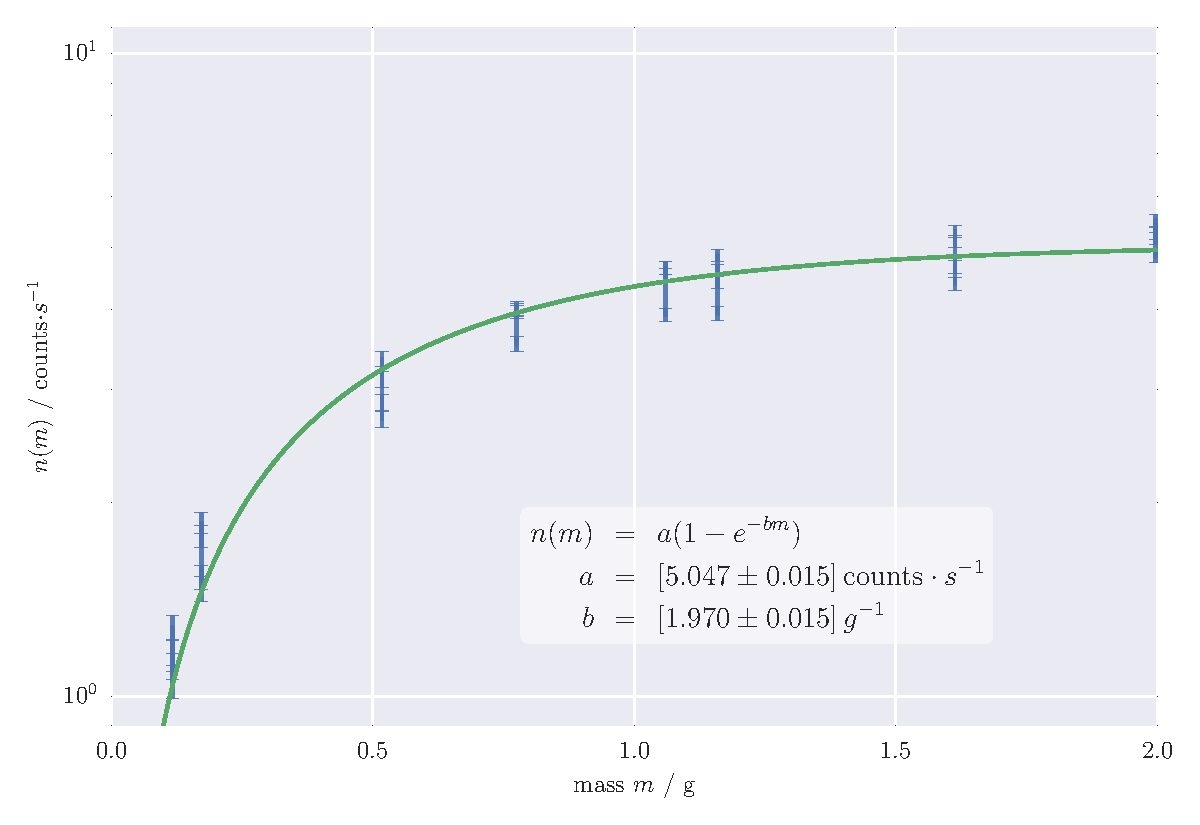
\includegraphics[width=\linewidth]{analysis/figures/measurement_2_4}
    \caption{Measurement 2.4 of potassium (with subtracted background, see table~\ref{tab:background_night1}) with various masses
    and the least squares fit of the data. The error for the difference
    of signal and background is $s_n = \sqrt{\frac{n_{sam.}}{t_{sam.}}+\frac{u_{back.}}{t_{back.}} }$, see see equation \eqref{eq:error_sam} for
    the derivation of the error.}
    \label{fig:2_4_potassium}
\end{figure}
\subsubsection{Least squares fit}
In the theory part, subsection~\ref{subsec:potassium} we explained the 
behavior of the counting rate in dependence of the mass with
equation \eqref{eq:potassium}
\begin{equation*}
n(m) = f_B \frac{\Omega}{4 \pi} A_s \frac{F \rho }{\mu}A \left (1 - \exp \left ( - \frac{\mu}{F \rho}m \right ) \right ).
\end{equation*}
The least squared algorithm yielded the following result
\begin{eqnarray}
    \mathrm{cov}(a,b) &=& 
    \begin{pmatrix}
        0.00021 &-0.00018 \\
        -0.00018 &0.00023 \\
    \end{pmatrix}\\
 \Rightarrow \qquad
    a &=& \left [ 5.047 \pm 0.015 \right ] \text{counts} \cdot s^{-1} \\
    b &=& \left [ 1.970 \pm 0.015 \right ] g^{-1} \\
    \chi^2/\mathrm{dof} &=& 2.869 
\end{eqnarray}
The $\chi^2/dof$ is not 1, but it is not far away. Since the number of measurements is not impressively high, we
can assume that the $\chi^2/dof$ is in an order of magnitude to accept the model (as its functionality is at this
dimension also limited). The correlations are of the same order of magnitude as the errors, so we can conclude that
the variables are rather strongly correlated.
Since $a$ and $b$ are correlated, we have to use the correlation matrix for
error propagation. We can use the convient formula \eqref{eq:pot_final} derived
in the theory section in subsection~\ref{subsec:potassium}
\begin{equation*}
T_{1/2} = \frac{\eta}{a b} = [3.82\pm0.13]\cdot 10^{16} s = [1.21 \pm 0.04]\cdot 10^9 a
\end{equation*}
with $\eta = [3.80 \pm 0.06]\cdot 10^{17}$ counts/g, which we derived before.\\
The literature value is $T_{1/2} = [1.248 \pm 0.003]\cdot10^9$a, which is within the range of our result. 

